\subsection{Related Work}
\label{sec:sec_relapp}
Various approaches leverage the potential of machine learning methods for knowledge extraction. Our work resides in the field of distributed computation of the $k$-nearest neighbors joins over Big Data and its extension to perform several machine learning tasks. In the following, we present a review of the relevant literature.

% $k$NN and machine learning
Several works in the literature have reported the superiority of $k$-nearest neighbors on machine learning tasks over similar approaches, both in terms of processing time, as well as in terms of accuracy~\cite{amancio2014systematic, yang1999evaluation, colas2009data}. There are numerous approaches that exploit its potential. Zhang et al.~\cite{linkg2005multi} introduced a multi-label classification method based on $k$NN which uses a \textit{Maximum a Posteriori} (MAP) principle to predict the class of an new element. Oswald et al.~\cite{oswald2001traffic} used an approximate $k$NN-based regression approach in order to forecast traffic flow. Wei and Keogh~\cite{wei2006semi} presented that an $1$NN classifier outperforms other similar methods in terms of error rate, when applied on time-series data. Xu~\cite{Xu2011mwk} introduced a multi-label weighted $k$NN classifier, where the weights for each class are computed via mathematical optimization, using Least Squared Errors (LSE). Gou et al.~\cite{Gou2011jcp} presented a weighted voting scheme for such classifiers, where the distance between an element and its nearest neighbors determines the weight of each neighbor's vote. The query element is classified to the most weighted class. In our approach, we extend this functionality by also calculating the probability of each element belonging to each class. Also, by employing a $k$-nearest neighbors joins approach, we allow for simultaneous classification or regression on datasets of really high volume, addressing the challenges that arise when processing Big Data in a distributed environment.

% Dimensionality reduction and Space Filling Curves
Similarly to many data analysis and management tasks, $k$NN joins suffer from the \textit{curse of dimensionality}~\cite{berchtold1998his}. Liao et al.~\cite{liao2001SFC} stated that as the number of dimensions increases, such techniques need an exponentially larger amount of CPU time. Consequently, executing a $k$NN joins method on Big Data requires prohibitively long-lasting operations. To overcome this issue, \textit{dimensionality reduction} can be applied on the datasets by indexing their elements via a \textit{Space Filling Curve} (SFC)~\cite{sagan2012space}. This approach reduces data dimensionality to one dimension, which allows for a significantly faster execution of an approximate nearest neighbor search, based on the indexed elements. The most widely used SFCs are the \textit{$z$-order}, \textit{Gray-code} and \textit{Hilbert}, among which Mokbel et al.~\cite{mokbel2002pms} concluded that Hilbert is the most ``fair'', due to the fact that two consecutive points in the curve are always nearest neighbors. Yao et al.~\cite{yao2010knn} used the $z$-order curve to significantly boost the query performance over huge amounts of data. Lawder et al.~\cite{lawder2001qmd} efficiently executed range queries in data indexed by the Hilbert curve, while Faloutsos~\cite{faloutsos1986mhu} presented a mathematical model for indexing the multi-attribute records of a data collection, using Gray-codes instead of binary values. Similarly, Chatzigeorgakidis et al.~\cite{chatzigeorgakidis2015mapreduce} and Zhang et al.~\cite{zhang2012epk} exploit the $z$-order curve in order to perform $k$NN joins on a distributed environment. To support selection variety, the proposed framework can operate by tuning and using the most preferable among these SFC methods, as space traversal quality and computation performance may differ according to the data context. Figure~\ref{figure1} shows an example of the recursive way the three SFCs scan the elements in a two-dimensional space.

% Figure 1 should go here
\begin{figure}[h!]
	\centering
	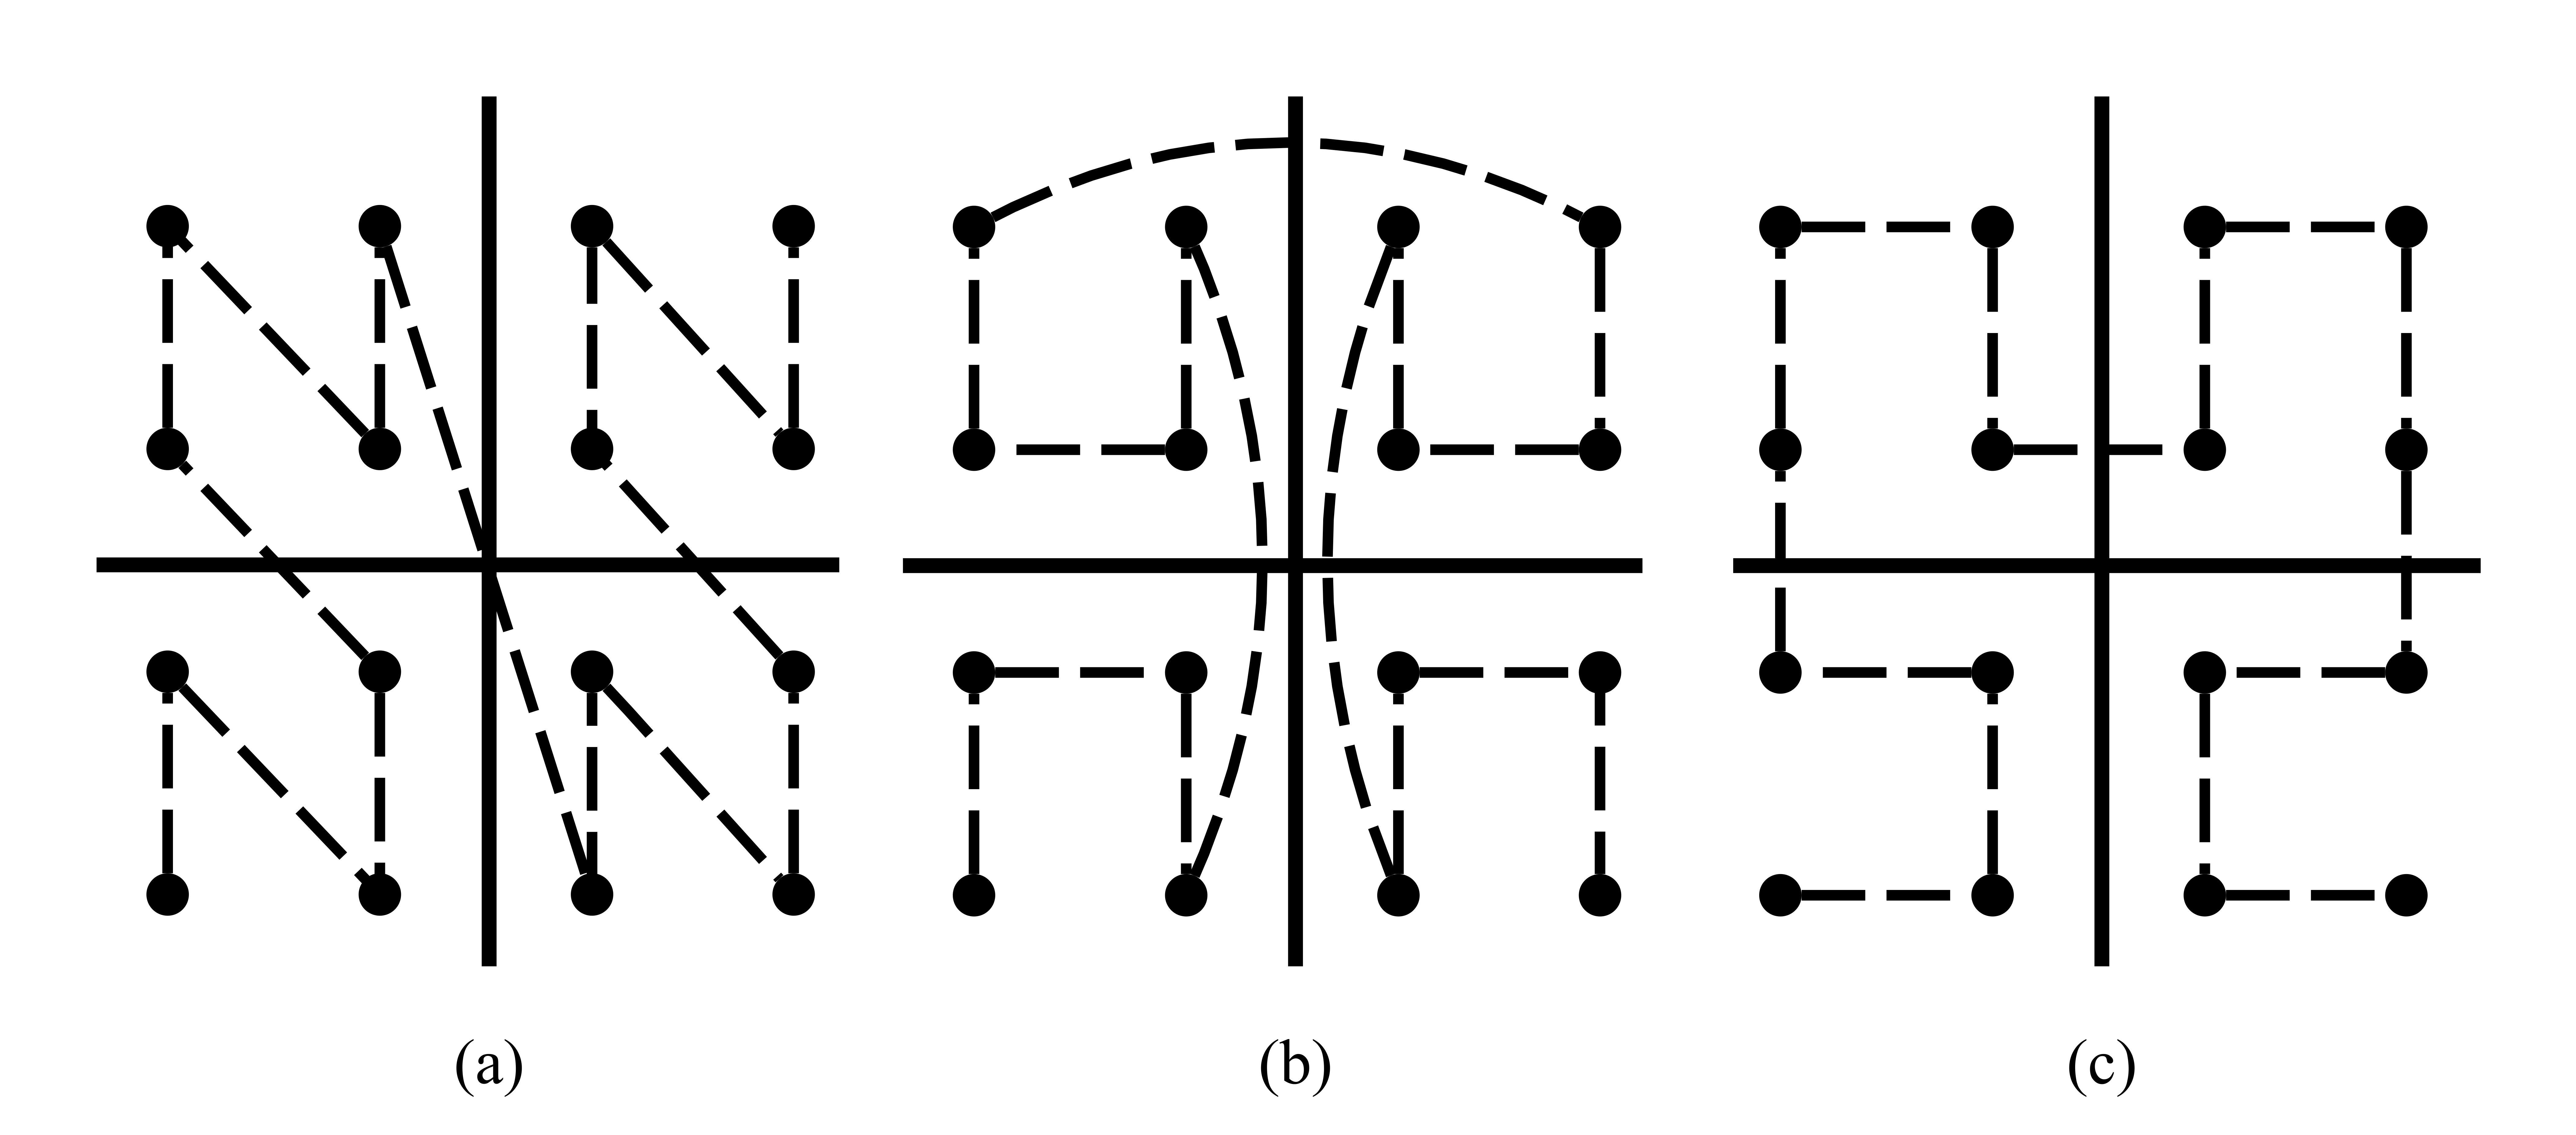
\includegraphics[width=\textwidth]{figures/figure1.png}
	\caption{The three Space Filling Curves. Μore particularly, (a) $z$-order curve, (b) Gray-code curve (c) Hilbert curve.}
	\label{figure1}
\end{figure}

% $k$NN on distributed environments
The increasing scientific interest in the Big Data area has introduced modern distributed implementations of famous algorithms. More particularly, several approaches of MapReduce-based $k$NN joins algorithms have been proposed. Song et al.~\cite{song2015hal} present a review of the most efficient among them, denoting that all share the same three processing stages, i.e., (i) \textit{data pre-processing}, (ii) \textit{data partitioning and organization}, and (iii) \textit{$k$NN computation} stage. They conclude that the SFC-based H-$zk$NNJ~\cite{zhang2012epk} algorithm, outperforms in terms of completion time other similar methods like \textit{RankReduce}~\cite{stupar2010rankreduce}, which uses \textit{Locality Sensitive Hashing} (LSH)~\cite{indyk1998ann}. Chatzigeorgakidis et al.~\cite{chatzigeorgakidis2015mapreduce} extended the functionality of H-$zk$NNJ~\cite{zhang2012epk}, by delivering the F-$zk$NN probabilistic classifier, which performs classification on the results of a $k$NN joins query. The F-$zk$NN probabilistic classifier is based on the MapReduce programming model and executed in a single distributed session. However, the datasets need to be propagated between the first two execution stages using local caches, which results in increased communication costs. Our approach optimizes F-$zk$NN by avoiding this costly propagation using Flink's broadcast sets and augments its functionality by incorporating an additional regression analysis operation. Both the probabilistic classifier and the regressor are included in a wider distributed processing framework and are experimentally applied on water consumption related Big Data analysis tasks.

% $k$NN in resources consumption domain
Similar approaches which apply machine learning methods on resource consumption data (e.g., energy, water) but still not from a Big Data perspective, include the work of Chen et al.~\cite{chen2011aab} who used a $k$NN classification method and labeled water data to identify water usage. Naphade et al.~\cite{swp2011} and Silipo and Winters~\cite{bdse2013} focused on identifying water and energy consumption patterns, providing analytics and predicting future consumptions but in high granularity levels and in small scale. Schwarz et al.~\cite{schwarz2012lpss} used $k$NN for classification and short-term prediction in energy consumption by using smart meter data, however, they focused on in-memory and non-distributed approaches, thus, limiting the applicability on larger datasets. Our approach partially relates to the work of Kermany et al.~\cite{Kermany2013aam}, where the $k$NN algorithm was applied for classification on water consumption data, in order to detect irregular consumer behavior. We take a step forward by applying our algorithm on two real-world case studies, delivering predictive analytics for water consumption in a Big Data scale.